\chapter{IBM BigFix on SaaS, l'implementazione del prototipo}
L'attenta progettazione giudata dall'architect che abbiamo visto nel capitolo precedente è servita da base per la vera ralizzazione del prototipo che rappresenta l'aspetto implementativo del progetto BigFix SaaS. Ma queste due fasi del lavoro che stiamo presetando non sono l'una successiva l'altra. Infatti è bene rimarcare che, sguendo un approccio agile, iterativo e incrementale, l'intero disegno del progetto si è ottenuto solamente a fronte di una continua esplorazione dei requisiti che si è protratta durante tutta la fase implementativa. Il metronomo dello sviluppo sono state infatti le sprint demo, le quali vedevano la partecipazione anche di altri stackeholders interni all'azienda, oltre che al team stesso. Da questi confronti sono risultati continui feedback che hanno contribuito a portare il lavoro nel suo stato attuale.

\section{Container e microservizi di BigFix}
Per la necessità di continui feedback già dalla prima fase del progetto si è scelto di adottare, per i primi sprint, una soluzione intermedia per quanto riguarda la scomposizione del prodotto nei container. Si deciso infatti di fare in modo che, all'inizio, ogni container ospitasse un realay o un server di uno dei clienti forniti dal SaaS, e non un microservizio vero e proprio del prodotto. Questa scelta è avvenuta dopo un analisi dei requisiti. Scomporre BigFix in microservizi è un'operazione che richiede molte ore uomo di lavoro e affrontarla all'inizio del progetto non avrebbe consentito ti testare nelle primissime fasi le tecnologie che si erano individuate per il deployment. Avendo presto a disposizione gli ambienti cliente con relay e server, si sono subito testati scenari tipici del prodotto on premises nelle nuove tecnologie SaaS adottate.

\section{Gli ambienti di sviluppo }
La realizzazione di un progetto aziendale richiede più ambienti nei quali, sequenzialmente, viene testato il prodotto prima di metterlo sul mercato. L'ambiente ufficiale, quello di produzione, deve garantire tutti i parametri qualitativi di cui abbiamo parlato precedentemente. Per questo motivo è lì che si concentrano i maggiori investimenti a livello hardware per garantire alte prestazioni al servizio. Al tempo stesso però occorre avere a disposizione un "laboratorio" in cui sviluppare e testare il software, in cui implementare le nuove features quando il prodotto sarà già sul mercato, un ambiente nel quale le modifiche che si compiono al codice non impattino in nessun modo il servizio offerto ai clienti. Per questo motivo il primo contesto in cui si è andato a lavorare è l'ambiente di sviluppo. Un ambiente chiuso all'esterno dell'azienda, ma che al tempo stesso simulasse nella maniera più fedele possibile l'ambiente di produzione. A questi due si aggiunge un'ambiente intermedio di pre production, nel quale vengono svolti tutti i test qualitativi per verificare che il prodotto sia conforme ai parametri non funzionali stabiliti. 
\begin{figure}[h!]
	\centering
	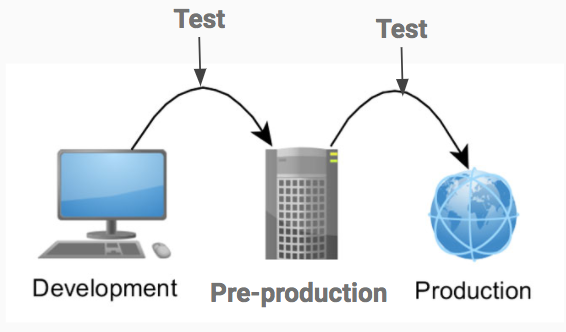
\includegraphics[width=0.7\textwidth,keepaspectratio=true]{capitoli/imgs/ambientisviluppo.png}
	\caption{Ambienti di BigFix SaaS}
\end{figure}

\section{Costruzione dell'ambiente e installazione di Docker e Kubernetes}
Vediamo una schematizzazione dell'ambiente di sviluppo nella figura \ref{ambs}. Kubernetes è il tool che muove le danze avendo proprio la funzione di orchestratore dei container. L'architettura di Kubernetes richiede che ci sia un nodo master che coordina i nodi denominati kube-node, che possono rappresentare macchine diverse. Su tutti i kube-node è installato anche docker, in quanto ci permetterà di ospitare su di essi i container. Questi vengono deployati su tutti i nodi a disposizione seguendo l'algoritmo di scheduling round-robin in modo da gestire al meglio le risorse di calcolo. 
\paragraph{}
Il Kubernetes master si interfaccia, come posiamo vedere, anche con altre due macchine presenti nella rete: La macchina DB2 e la macchina NFS. Andiamo a vedere di cosa si tratta.
\paragraph{DB2}
E' la macchina che ospita una replica del database. Spiegheremo in seguito come, nel processo di onboarding di un nuovo cliente, vengono dinamicamente allocate le risorse del database al nuovo utente. Le modalità di interazione tra i componenti BigFix nei container e il database ricalcano quelle del prodotto on premise.
\paragraph{Network File System (NFS)}
Questo componente è pensato per fornire storage per i container tramite protocollo NFS. L'NFS è un protocollo di rete sviluppato dalla Sun negli anni 80. Esso rappresenta un file system distribuito che consente ai computer di utilizzare la rete per accedere ai dischi rigidi remoti come fossero dischi locali. La componente NFS è stata utilizzata solamente in una prima fase del progetto in quanto, con il passaggio all'ambiente ufficiale, si è fatto affidamento allo storage fornito da un particolare componente di Kubernetes, il service. 

\begin{figure}[h!]
	\centering
	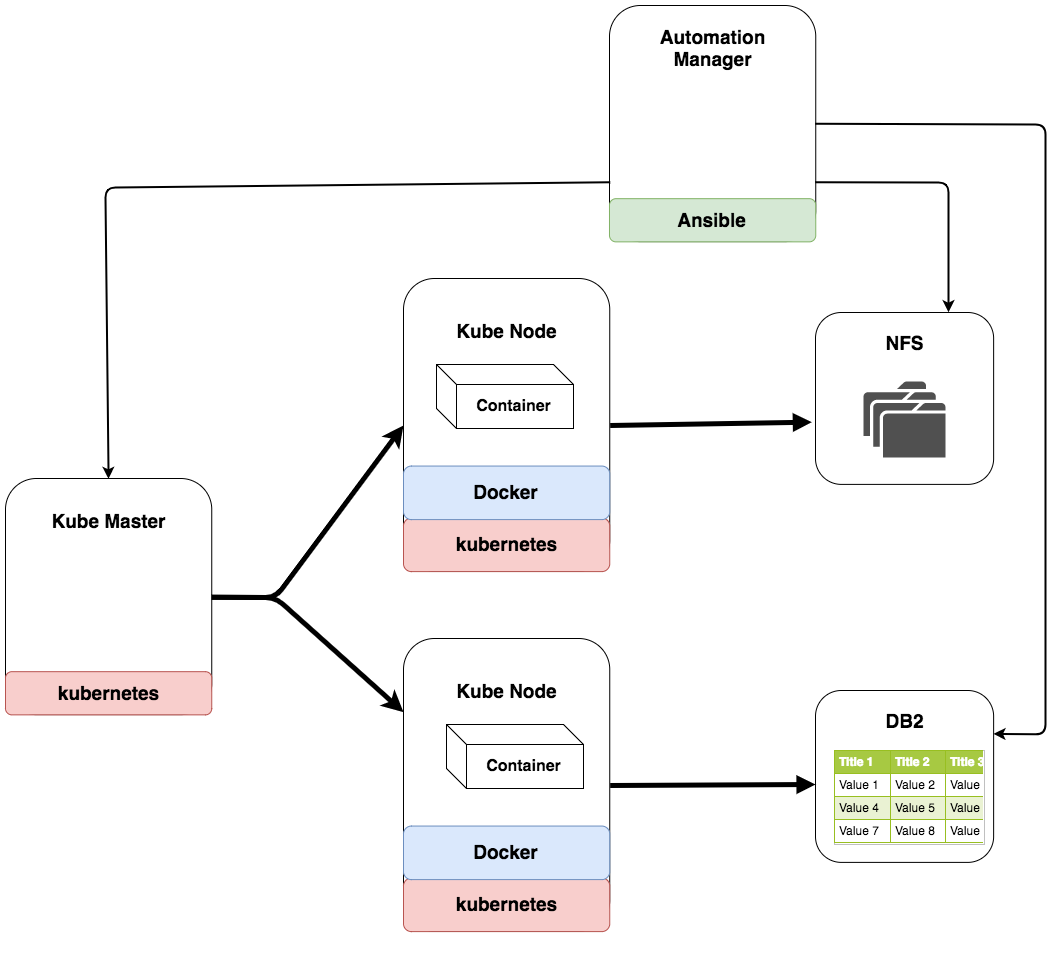
\includegraphics[width=0.5\textwidth,keepaspectratio=true]{capitoli/imgs/EnvironmentsComponentDiagram.png}
	\caption{L'ambiente di sviluppo di BigFix SaaS}
	\label{ambs}
\end{figure}


\section{Re-working degli installer del server e del relay di BigFix}
Il server e il relay di BigFix hanno i loro tradizionali installer relativi alla versione on premise del prodotto. Ovviamente è stato necessario un grosso lavoro di re-working di questi componenti per fare in modo che risultassero molto più leggeri e adatti al deployment in un container.

\section{Le immagini Docker}
Docker consente di deployare i container partendo da immagini di una repository fornita da Docker stesso. Nel nostro caso si è scelto di porre come base di tutti i container del servizio una macchina Linux CentOS 7 sia per i relay che per i server, una scelta dettata da esigenze aziendali. Docker fornisce delle versioni a container di molti sistemi operativi in modo da personalizzare secondo le proprie esigenze i container che si vanno ad implementare.

\paragraph{}
Questa macchina CentOS è ovviamente una versione molto embrionale dei servizi necessari per il prodotto. E' stato necessario creare delle directory di BigFix apposite per ospitare l'installer del server o del relay, a seconda dei casi. Si sono poste poi, all'interno di opportune cartelle, due file bash fondamentali per il deployment: install.sh e start.sh. Nella prossima sezione spieghiamo il loro compito.

\section{Docker containers, Pods e services}
I file bash di cui abbiamo parlato nella sezione precedente vengono in realtà eseguiti in contesti differenti. Install.sh viene chiamato in causa da Docker che in questo modo installa appunto il container. Successivamente Kubernetes chiama start.sh e avvia a tutti gli effetti i servizi di server e relay.
\paragraph{}
Ora occorre porre l'accento su come i container interagiscono con Kubernetes. La scelta in questo progetto è stata quella di avere una corrispondenza biunivoca tra i container di Docker e i pod di Kubernetes in modo da avere una semplicità di gestione dei container stessi. Vi è inoltre un ulteriore livello di astrazione sopra i Pod. Kubernetes offre infatti la possibilità di utilizzare il componente Service, che raggruppa in se uno o più pod. In questo progetto è stato utilizzato con il fine di poter utilizzare il pod nella rete in maniera più efficiente.
\paragraph{Yaml} 
I pod di Kubernetes utilizzano un particolare linguaggio di serializzazione lo YAML (YAML Ain't Markup Language). Esso è per certi versi molto simile all'XML e al JSON, ma è molto più essenziale e quasi tutto il suo contenuto rappresenta il dato da serializzare. I suoi punti di forza sono la manutenibilità e la flessibilità. Un file JSON infatti è anche un file YAML valido. All'interno dei file YAML si sono configurati tutti gli aspetti dei pod che sono necessari a Kubernetes per far partire i servizi relay e server con la struttura desiderata. Vediamo nella figura \ref{fig:yaml} un esempio di configurazione per un pod.
\begin{figure}
	\centering
	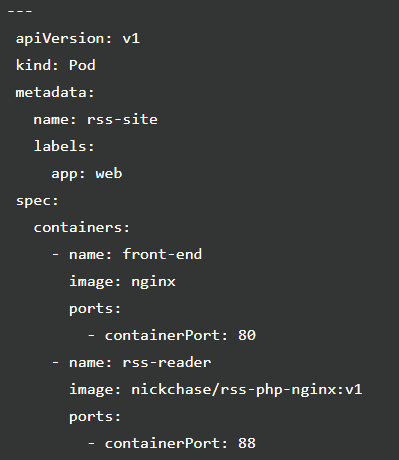
\includegraphics[width=0.5\linewidth]{capitoli/imgs/yaml}
	\caption{Esempio di YAML di configurazione per Kubernetes}
	\label{fig:yaml}
\end{figure}


\section{Modifiche al relay necessarie per la versione SaaS}
Il componente relay ha avuto bisogno di numerosi accorgimenti per permettere il suo funzionamento in prospettiva SaaS. Per sua natura, ha bisogno di numerose informazioni a riguardo del server al quale fanno riferimento. Per configurare il relay correttamente è necessario far rinvenire al relay alcuni file contenenti queste informazioni. Questa era una procedura che nella versione on premise veniva fatta a mano. Ora, nella realizzazione del servizio in SaaS, si è implementato un procedimento automatico che fa affidamento sullo storage condiviso fornito dall'NFS.
\paragraph{Relay scaling}
Altra proprietà del relay è la capacità di scalare adeguatamente rispondendo alle necessità. Durante il tipico utilizzo del prodotto è molto comune che il numero dei client o la mole di lavoro richiesta cambino dinamicamente. Superata una certa soglia di workload o un certo numero di client (circa 1000), un singolo relay non è più in grado di far fronte alle richieste, ma ha bisogno che parte dell'onere di lavoro venga presa in carico da una sua copia identica. Questo processo viene chiamato di "scale up". Analogamente possono verificarsi delle situazioni in cui le risorse allocate siano sovradimensionate rispetto al carico di lavoro. Fortunatamente Kubernetes fornisce un comando ad hoc per queste necessità. Questo strumento utilizza dei volumi condivisi di appoggio per fare si che le nuove copie dei relay non si debbano configurare da capo. Il nuovo relay infatti eredita dal primo sia tutte le configurazioni di BigFix e di Docker, ma anche la cache dell'altro relay, in maniera tale da essere subito operativo in pochi secondi. 
\paragraph{Air-gap}
Un'altro elemento che è necessario per abbattere i tempi per ottenere il nuovo relay funzionante è l'Air-gap. Senza scendere il dettagli e tecnicismi, questo componente ci consente di scaricare fixlet e altre configurazioni proprie di BigFix sul nuovo relay in tempi estremamente rapidi. 
\section{Automazione del Deployment}
Facciamo il punto della situazione cercando di individuare gli elementi che sono stati definiti fino a questo punto. Abbiamo da un lato la possibilità di deployare dei container che svolgano le funzioni di server o di relay perfettamente funzionanti, da un'altro c'è il database DB2 pronto a fornire persistenza a tutti i dati del cliente, da un'altro ancora altri componenti necessari all'ambiente per il corretto funzionamento, come l'NFS. Supponiamo che in un istante non predicibile un nuovo cliente acquisti la licenza ad utilizzare BigFix SaaS e abbia appena compilato la form con tutti i dati necessari. Cosa manca? 
\paragraph{}
Non è certo pensabile che a questo punto ci sia bisogno di un intervento umano per mettere a disposizione del nuovo cliente tutte le risorse necessarie. Ci si aspetta che il servizio sia disponibile nel giro di poche ore e la richiesta può essere avvenuta da qualunque parte del mondo e in qualunque momento della giornata.
\paragraph{}
Ecco quindi che è stato necessario un processo di software automation. Un processo automatico cioè che porti il prodotto ad essere pronto all'utilizzo da parte del nuovo cliente. Questo processo deve essere tollerante a malfunzionamenti e deve poter interagire con tutte le componenti facenti parte del sistema. Deve, in sostanza, comportarsi come una figura umana dedita all'istallazione. 

\subsection{Bash Scripting}
Nel progetto si è fatto largo uso del linguaggio Bash. Dovendo interagire con sistemi UNIX esso è stato spesso inserito in processi di automazione presenti negli scenari di gestione del sistema.
\paragraph{}
Bash, acronimo che sta per Bourne-Again-Shell, è un'interfaccia a riga di comando pensata per gestire i sistemi operativi UNIX nata alla fine degli anni '80. Come altri strumenti analoghi, oltre alla modalità interattiva, prevede anche la possibilità di creare script, con funzioni, cicli e costrutti tipici, e di eseguirli poi in blocco. Questi script sono contraddistinti dall'estensione .sh e dall'incipit "\#!/bin/bash", il quale indica il percorso della shell che dovrà eseguire lo script, Bash per l'appunto. 
\paragraph{Utilizzo degli script Bash nel progetto}
Gli script Bash sono stati di fondamentale importanza per il progetto. Data la loro versatilità e potenza è stato possibile utilizzarli per molti scopi di configurazione. Sono entrati, ad esempio, in dei flussi Ansible e Jenkins. Questi script venivano mandati tramite scp su opportune macchine e, una volta configurati i permessi, venivano eseguiti per svolgere i più disparati compiti necessari.
\subsection{Jenkins}
Il solo utilizzo di script bash non può garantire la corretta gestione di un'architettura così complessa come quella del SaaS di BigFix. Gli step di configurazione necessari ogni qualvolta si debba effettuare l'onboarding di un nuovo cliente sono numerosi e ripetitivi e quindi risulta molto utile adoperare un tool di automation.
\paragraph{}
Per questo motivo, almeno in un primo momento, si è utilizzato uno dei più diffusi strumenti di continuous integration: Jenkins. Esso è un progetto open-source nato da Oracle negli ultimi anni. Jenkins ci consente di eseguire e monitorare sistematicamente task ripetitivi come possono essere ad esempio i processi di building. Il sistema, disponibile tramite server web, ha la possibilità di essere integrato con innumerevoli plugin che lo rendono adatto a automatizzare i task più disparati sulle macchine più eterogenee. 
\paragraph{}
Nel lavoro di tesi si sono utilizzati proprio alcuni di questi plugin per permettere, a partire dalla macchina di Automation Manager in cui è installato, di orchestrare tutti i task sulle singole macchine dell'ambiente tramite ssh e scp.
\paragraph{}
Uno step preliminare che è stato necessario è quello di distribuire opportuni certificati alle macchine in modo da poter consentire la comunicazione tramite Jenkins. In questo modo non era più necessario esplicitare ogni volta la chiave ssh, ma si instaura una comunicazione a chiave pubblica e chiave privata. 
\paragraph{}
A questo punto necessario scrivere opportuni script bash per i diversi task che erano necessari per allocare le opportune risorse a ogni cliente.I tipici step necessari nelle diverse macchine del nostro ambiente sono i seguenti:
\begin{itemize}
	\item Creazione di opportune directory nell'nfs per ospitare file di configurazione.
	\item Validazione della licenza di utilizzo del servizio 
	\item Creazione e connessione al database per i dati dell'utente e configurazione dello stesso.
	\item Personalizzazione degli YAML relativi al server e al relay
	\item Creazione e avvio dei servizi del server
	\item Creazione e avvio dei servizi dei relay
\end{itemize}
\paragraph{}
Ovviamente per eseguire questi passaggi è necessario interagire con tutte le macchine dell'ambiente. Jenkins ha la responsabilità di guidare tutti questi passaggi e prendere opportune contromisure a eventuali malfunzionamenti. 
\begin{figure}[h]
	\centering
	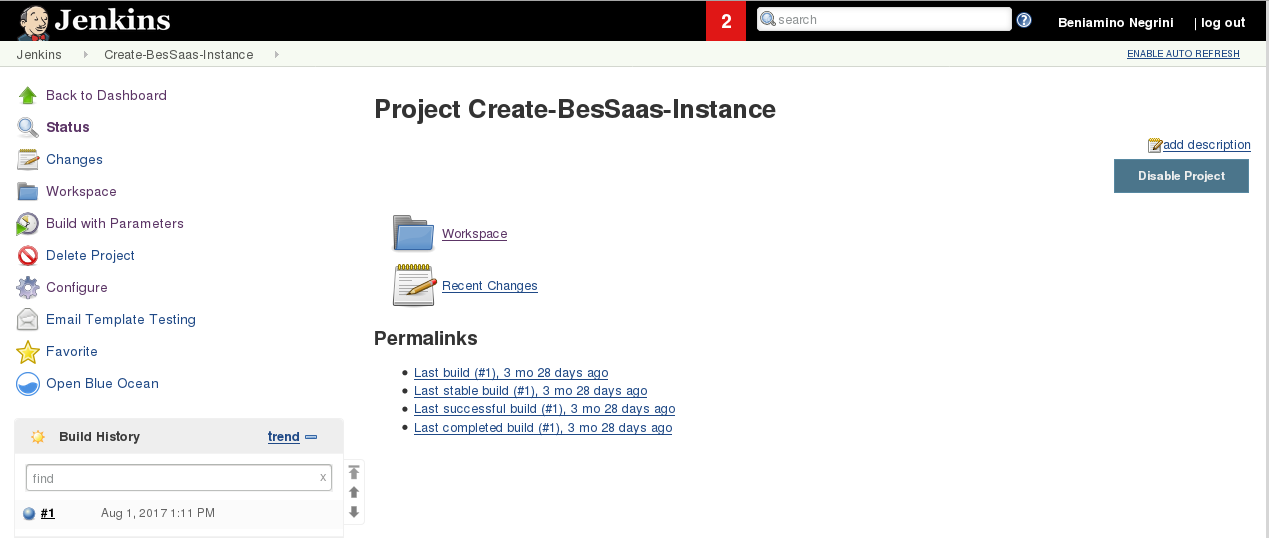
\includegraphics[width=0.7\linewidth]{capitoli/imgs/jenkisProj}
	\caption{Una delle schermate di configurazione di Jenkins}
	\label{fig:jenkisproj}
\end{figure}

\subsection{Ansible}
\paragraph{}
scrivere qui perchè si è passati ad ansible anzichè jenkins
\paragraph{}
Relativamente alle modalità di utilizzo che si sono fatte in questo progetto Ansible rappresenta un'alternativa all'utilizzo di Jenkins. Ansible è uno strumento di automation nato nel 2012. Il tool si basa su due tipi di componenti, le macchine controllori che fanno partire l'automation e i nodi che sono le macchine dove avvengono eseguiti i task. 
\paragraph{}
Nel progetto è stata sfruttata molto la modularità di Ansible che permettere di sfruttare le strutture dei playbook e dei roles. Sostanzialmente un role è una successione di determinati task che hanno un fine e un target comune. I playbook sono delle collezioni di roles, i quali vengono così assemblati a piacimento per ottenere le configurazioni desiderate, come nel caso dell'ambiente di BigFix SaaS. 
\subsection{UrbanCode Deploy e code promotion}
C'è ancora un tool che è necessario integrare per garantire continuous integration e continuous delivery. Teniamo per un attimo in mente gli ambienti di sviluppo di cui abbiamo parlato nella sezione 7.2. Sarebbe molto utile che, ogni qualvolta viene effettuata una modifica al codice, un processo automatico integri questa modifica sequenzialmente negli ambienti di development, pre-production e production. Il passaggio tra questi ambienti può essere automatizzato ponendo come condizione di promozione all'ambiente successivo opportuni test automatici. Questo processo è chiamato di code promotion. 
\paragraph{}
Il tool in questione è un prodotto di IBM chiamato UrbanCode Deploy. Esso consente di coordinare e automatizzare le implementazioni delle applicazioni, le configurazioni di middleware e le modifiche ai database in ambienti di produzione e di test on-premise o basati su cloud. Nel progetto di tesi UrbanCode monitora l'esito dei playbook di Ansible e, in base al loro esito, decreta se fare o meno code promotion.
\begin{figure}
	\centering
	
\includegraphics[width=0.7\linewidth]{capitoli/imgs/ucd}
	\caption{IBM UrbanCode Deploy}
	\label{fig:ucd}
\end{figure}

\section{Scenario di onboarding di un nuovo cliente}
corregere immagine bern
\section{Scenario di upgrade del servizio}

\section{Automazione del Testing}
\subsection{Functional Test}
\subsubsection{JUnit}
\subsubsection{JUTAA}
\subsection{Security Test}
\subsubsection{AppScan}
\subsubsection{Image Compliance}
\subsection{Performance Test}
\subsection{Penetration Test}
\subsection{Rielaborazione degli output del testing}

\section{Scenario di testing}

\section{Il passaggio all'ambiente di produzione}
kubernetes -> ip pubblico, dns


